
% vim: set ts=4 sw=4 tw=80 noexpandtab:
%******************************************************************************%
%                                                                              %
%                   Machine_Learning_03.tex                                    %
%                   Made by: ikourkji                                          %
%                                                                              %
%******************************************************************************%

\documentclass{42-en}

%******************************************************************************%
%                                                                              %
%                                   Prologue                                   %
%                                                                              %
%******************************************************************************%

\begin{document}

\title{Introduction to Machine Learning}
\subtitle{Linear Regression}

\member {Jeson}{ljunzhen@42.us.org}
\member {}{Jesonleejunzhen.com}

\summary
{
Learn the most basic type of regression model, linear regression! 
}

\maketitle

\tableofcontents

%Initialisation des headers d'exercices

\newpage

\bigskip

\centerline{
\includegraphics[width=150mm]{images/dontpanic.png}}

\centerline{\texttt{Eat, Sleep, Code, Repeat.}}

%******************************************************************************%
%                                                                              %
%                           What is Linear Regression?                         %
%                                                                              %
%******************************************************************************%

\chapter{Concepts of Linear Regression}
\section*{What is linear regression?}

Simple Linear regression is the most basic machine learning algorithm. Linear regression in simple terms is a statistical way of measuring the relationships between variables. Such as: as time increases, so does cost. It assesses how successfully a predictive variable does its job in predicting the outcome variable. It operates under the assumption that the two variables form a linear relationship.\\

There are two types of linear regression - Simple and Multiple.\\

\centerline{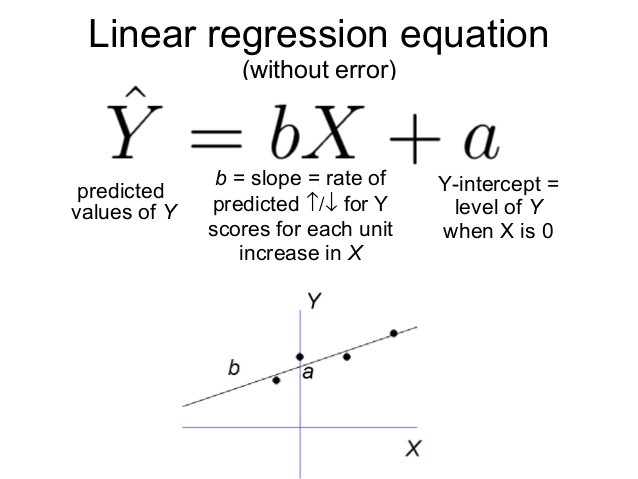
\includegraphics[width=150mm]{images/multiple-linear-regression.jpg}}

\section*{Cost Function}

Cost functions are a way to determine how well the machine learning model has performed given the different values of each parameter. We can measure the accuracy of our hypothesis function by using a cost function. This takes an average difference (actually a fancier version of an average) of all the results of the hypothesis with inputs from Xs and the actual output Ys.\\

The cost function will be the sum of the least square methods.\\

\centerline{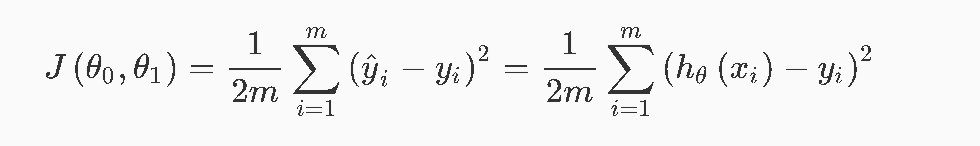
\includegraphics[width=150mm]{images/costFunction.png}}

\centerline{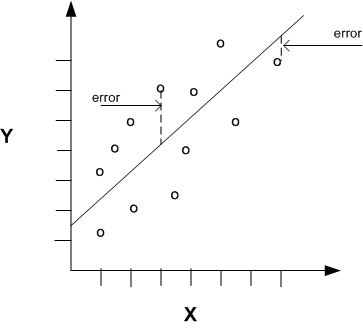
\includegraphics[width=125mm]{images/cost_graph.png}}

This function is otherwise called the "Squared error function", or "Mean squared error". But how do find the best fitting line with the smallest possible value of squared error function? We will talk about that later.\\

\section*{Gradient Descent}


Gradient descent is an optimization algorithm that finds the optimal weights (a,b) that reduces prediction error. In simple terms, gradient descent helps find the best fitting line with the minimum error through iterative steps. In the picture below, try guessing which color of the line has the minimum error?\\

\centerline{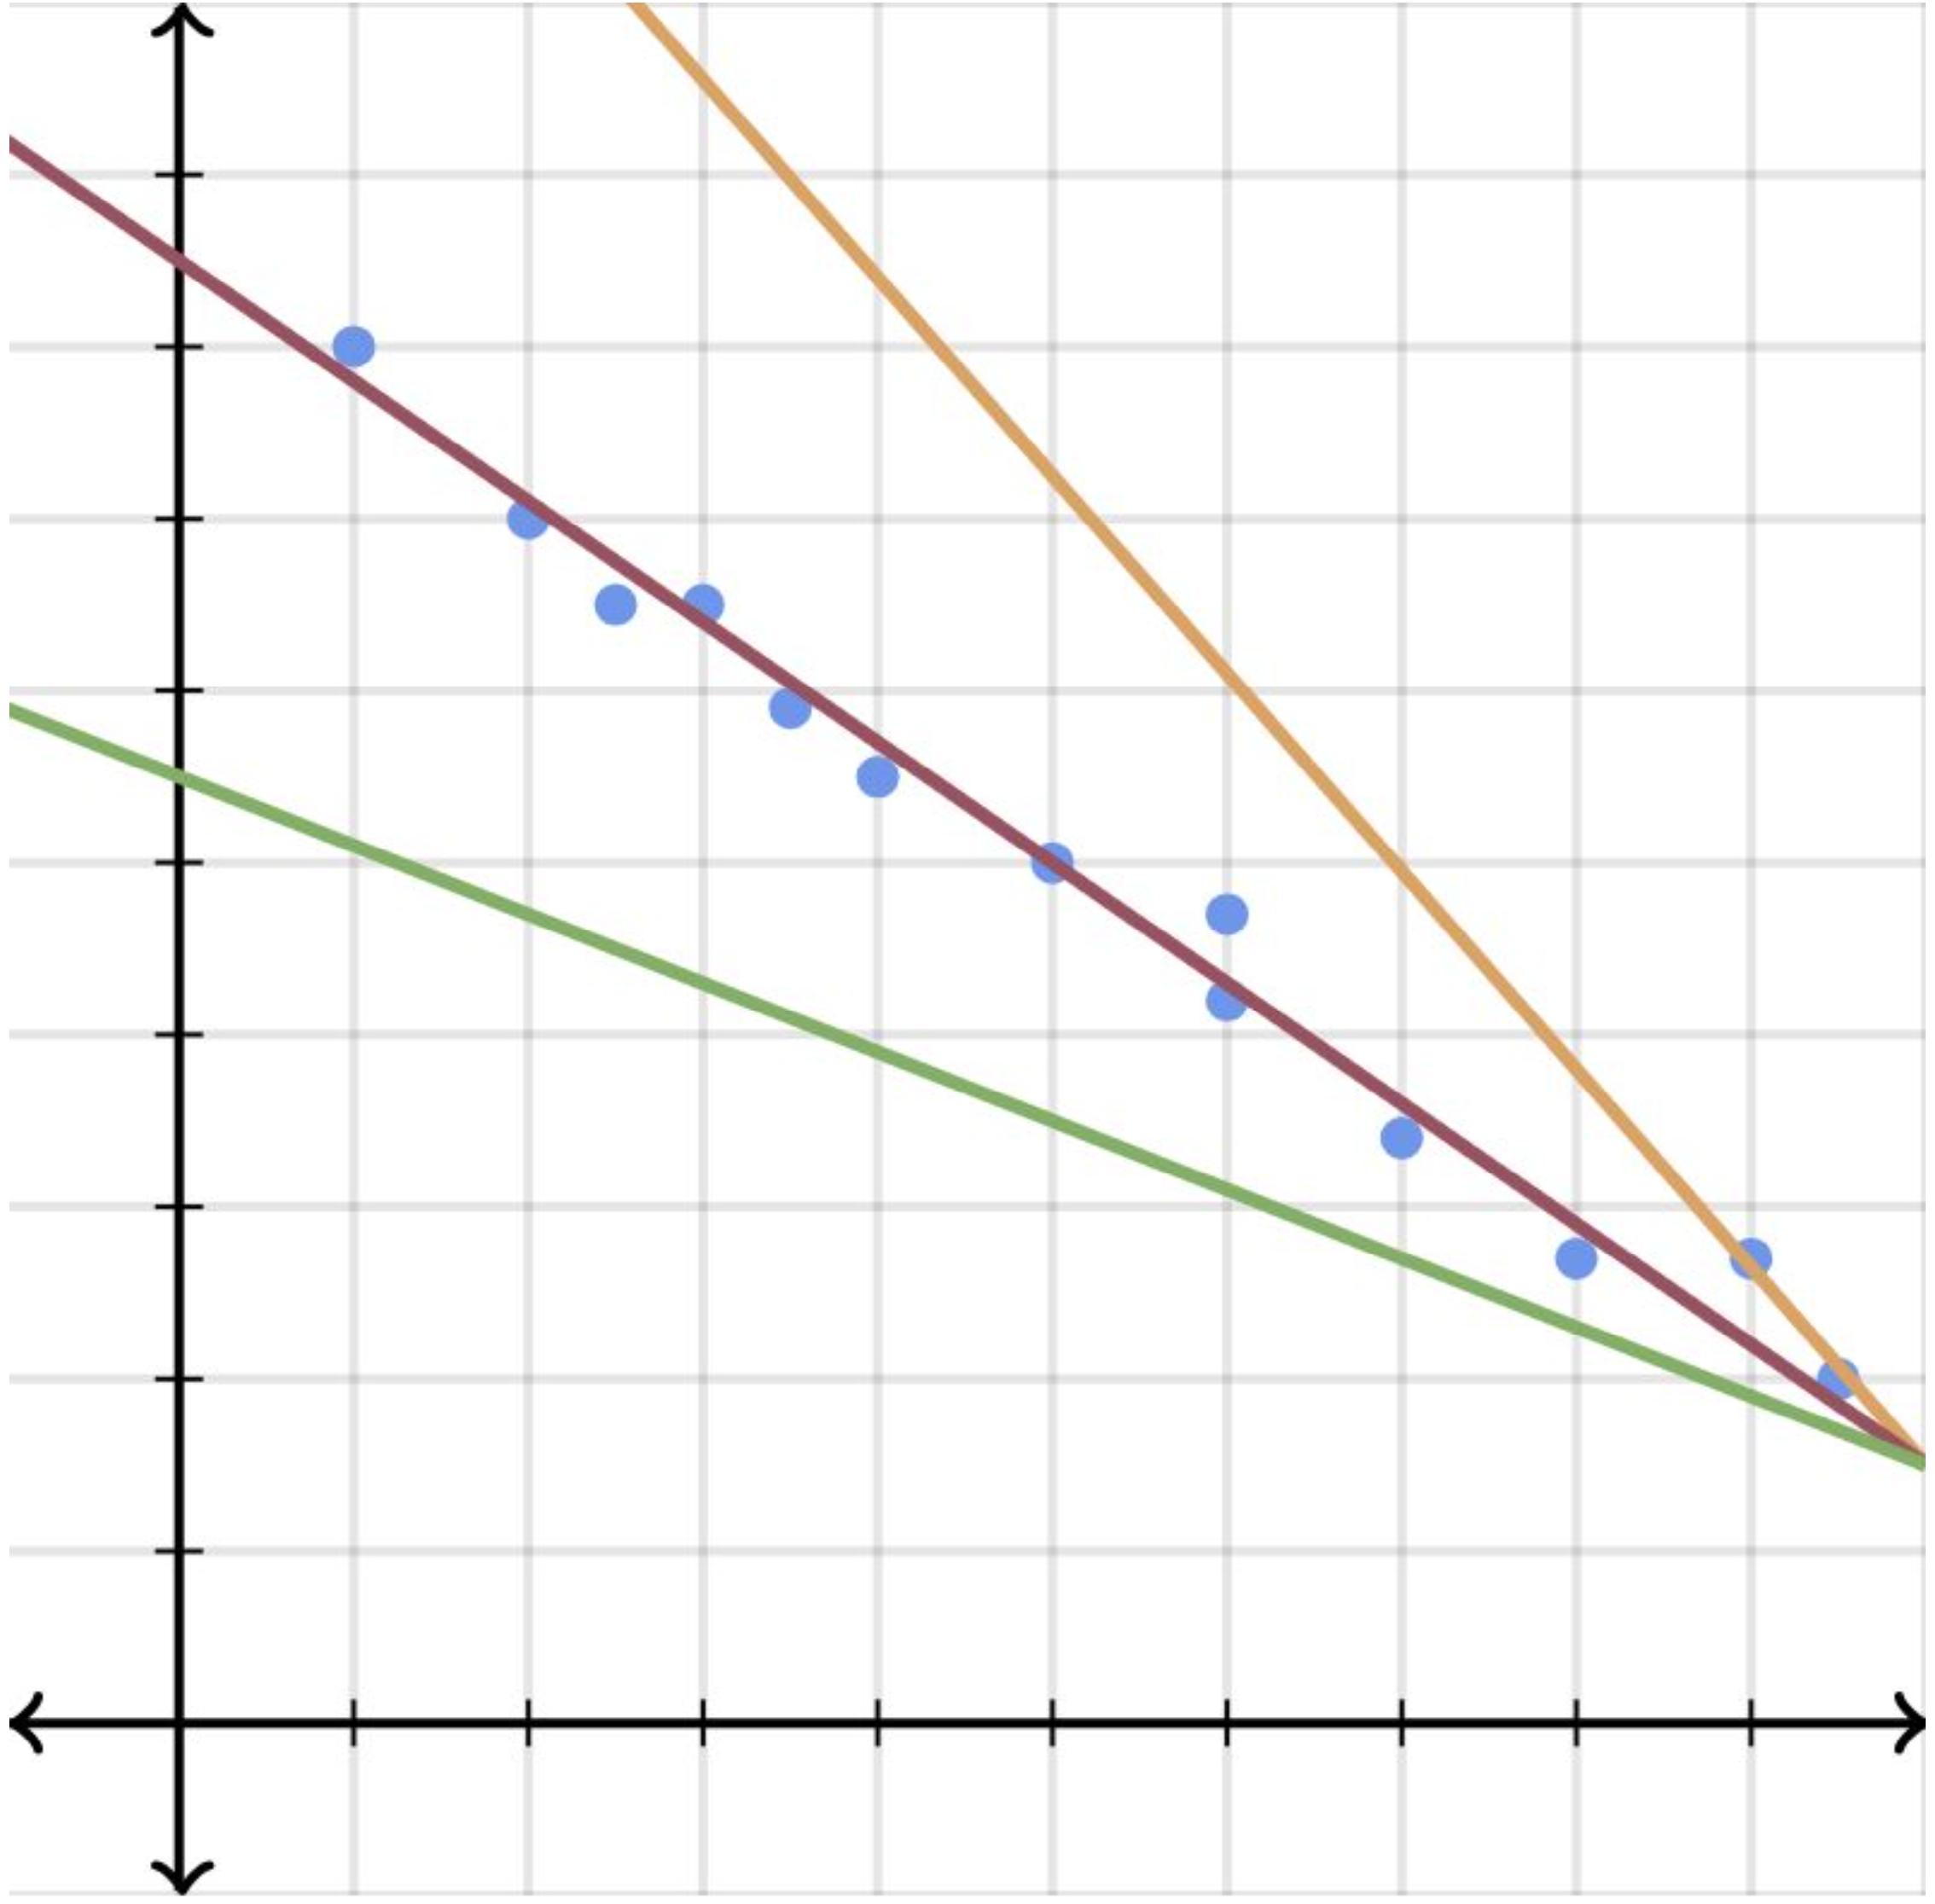
\includegraphics[width=100mm]{images/grad_pretty.png}}

Given a function defined by a set of parameters, gradient descent starts with an initial set of parameter values and iteratively moves toward a set of parameter values that minimize the function. This iterative minimization is achieved using calculus, taking steps in the negative direction of the function gradient.\\

\centerline{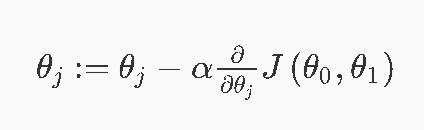
\includegraphics[width=125mm]{images/gradientDescent.png}}

\centerline{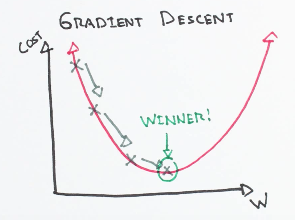
\includegraphics[width=100mm]{images/gradient_descent_demystified.png}}

We make steps down the cost function in the direction with the steepest descent. The size of each step is determined by the parameter α, which is called the  learning rate. Learning rate gives the rate of speed where the gradient moves during gradient descent. Setting it too high would make your path unstable, too low would make convergence slow. Putting it to zero means your model isn't learning anything from the gradients.  The lower the value, the slower we travel along the downward slope.\\

\centerline{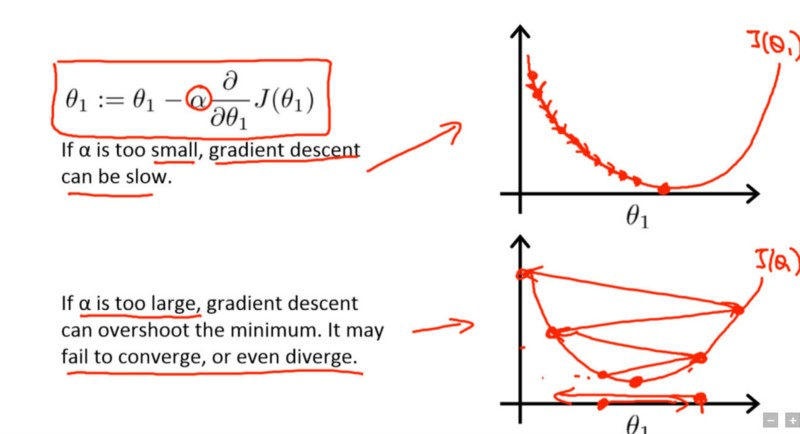
\includegraphics[width=150mm]{images/cost_grad_info.png}}

Play with this interactive page to understand learning rate better:\\
\href{https://developers.google.com/machine-learning/crash-course/fitter/graph}{https://developers.google.com/machine-learning/crash-course/fitter/graph}

\section*{Variants of Gradient Descent}

Do you know that there are different types of gradient descent? The main difference between them is the amount of data we use when computing the gradients for each learning step. The trade-off between them is the accuracy of the gradient versus the time complexity to perform each parameter update (learning step).
Let’s discuss the three variants of gradient descent algorithm:
\subsection*{Batch Gradient Descent}
Sum up overall examples on each iteration when performing the updates to the parameters\\
\subsection*{Mini-batch Gradient Descent}
A mini-batch is typically between 10 and 1,000 examples, chosen at random. Mini-batch SGD reduces the amount of noise in SGD but is still more efficient than full-batch.\\
\centerline{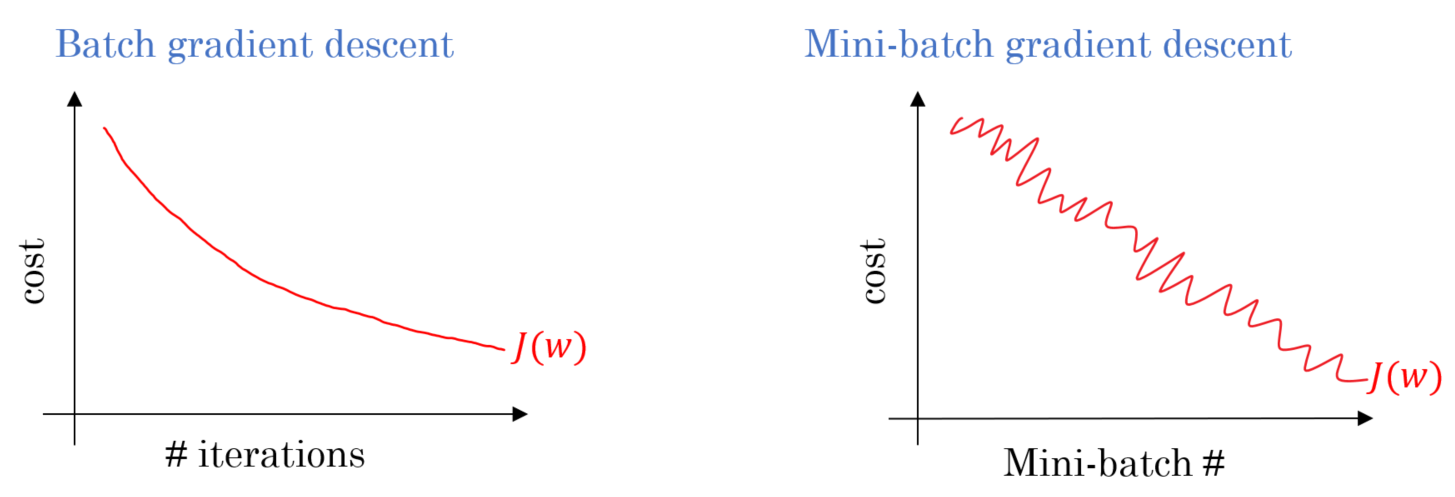
\includegraphics[width=150mm]{images/batch_grad_desc.png}}
\subsection*{Stochastic Gradient Descent}
Uses only a single example (a batch size of 1) per iteration. Given enough iterations, SGD works but is very noisy. The term "stochastic" indicates that the one example comprising each batch is chosen at random.\\
\centerline{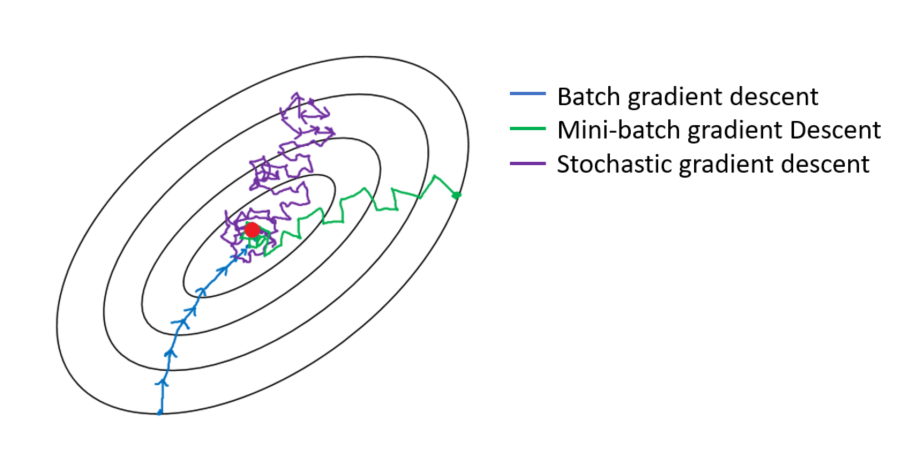
\includegraphics[width=150mm]{images/batch_disc.png}}

\section*{More information!}

\begin{itemize}
    \item Linear Regression:
    \begin{itemize}
        \item \href{https://medium.com/datadriveninvestor/machine-learning-model-simple-linear-regression-dbedb22ce200}{Machine Learning Model: Simple Linear Regression}
        \item \href{https://towardsdatascience.com/linear-regression-in-real-life-4a78d7159f16}{Linear Regression In Real Life}
    \end{itemize}
    \item Cost Function:
\begin{itemize}    
        \item \href{https://medium.com/@lachlanmiller_52885/machine-learning-week-1-cost-function-gradient-descent-and-univariate-linear-regression-8f5fe69815fd}{Machine Learning week 1: Cost Function, Gradient Desce, and Univariate Linear Regression}
        \item \href{https://medium.com/@lachlanmiller_52885/understanding-and-calculating-the-cost-function-for-linear-regression-39b8a3519fcb}{Understanding and Calculating the Cost Function for Linear Regression}
    \end{itemize}
    \item Gradient Descent:
    \begin{itemize}
        \item \href{https://towardsdatascience.com/gradient-descent-in-a-nutshell-eaf8c18212f0}{Gradient Descent in a nutshell}
        \item \href{https://spin.atomicobject.com/2014/06/24/gradient-descent-linear-regression/}{An Introduction to Gradient Descent and Linear Regression}
    \end{itemize}
    \item Variant of Gradient Descent:
    \begin{itemize}
        \item \href{https://towardsdatascience.com/gradient-descent-algorithm-and-its-variants-10f652806a3}{Gradient Descent Algorithm and Its Variants}
        \item \href{https://medium.com/@sunil.jangir07/variants-of-gradient-descent-5f5464c82f28}{Variants of Gradient Descent}
    \end{itemize}
    \item The first week of \href{https://www.coursera.org/learn/machine-learning}{Andrew Ng’s Machine Learning course on Coursera}
\end{itemize}

%******************************************************************************%
%                                                                              %
%                               Ask your peers                                 %
%                                                                              %
%******************************************************************************%
\chapter{Ask Your Peers}

\begin{enumerate}
    \item Explain what is a linear regression for and what kind of machine learning does it fall under?
    \item What can we use linear regressions for? Give 3 examples.
    \item Explain about cost function and the means squared error
    \item Explain gradient descent
    \item What is the difference between global and local minima?
    \item What is a learning rate? Does it matter if we have a large or small learning rate?
    \item What is the difference between mini-batch and stochastic gradient descent? What are the advantages and disadvantages of both?
\end{enumerate}

Read more on Google if you aren't able to answer these questions with confidence!

\startexercices


%******************************************************************************%
%                                                                              %
%                          Linear Regression Project                           %
%                                                                              %
%******************************************************************************%

\chapter{Exercise 00: Linear Regression Project}

\exfiles{salary.py}
\extopics{Linear Regression, scikit-learn, pandas, numpy, matplotlib}
\turnindir{Linear\_Regression}
\extitle{Linear Regression Project}
\makeheaderfiles

\section*{Scenario:}

Imagine you’re looking for a job as a software engineer. And you spotted a company that you want to work for. You already have 4 years of experience working as a developer, and you want to see how much you can make working in this company based on the number of years of experience you have.\\
Well, the good news is you have a dataset of the salary of all the employees in the company and their number of years of experience respectively. This is the perfect opportunity to apply linear regression to predict your salary!
You must be able to visualize the result with a scatter plot by using Matplotlib library. The image below is the end result of the test set that is expected to be displayed.\\
Using a \textbf{Jupyter notebook} to build this project will be highly recommended. Download the dataset to begin. Happy hacking!

\hint{Use the \href{https://scikit-learn.org/stable/}{scikit-learn library} to perform linear regression.}

\centerline{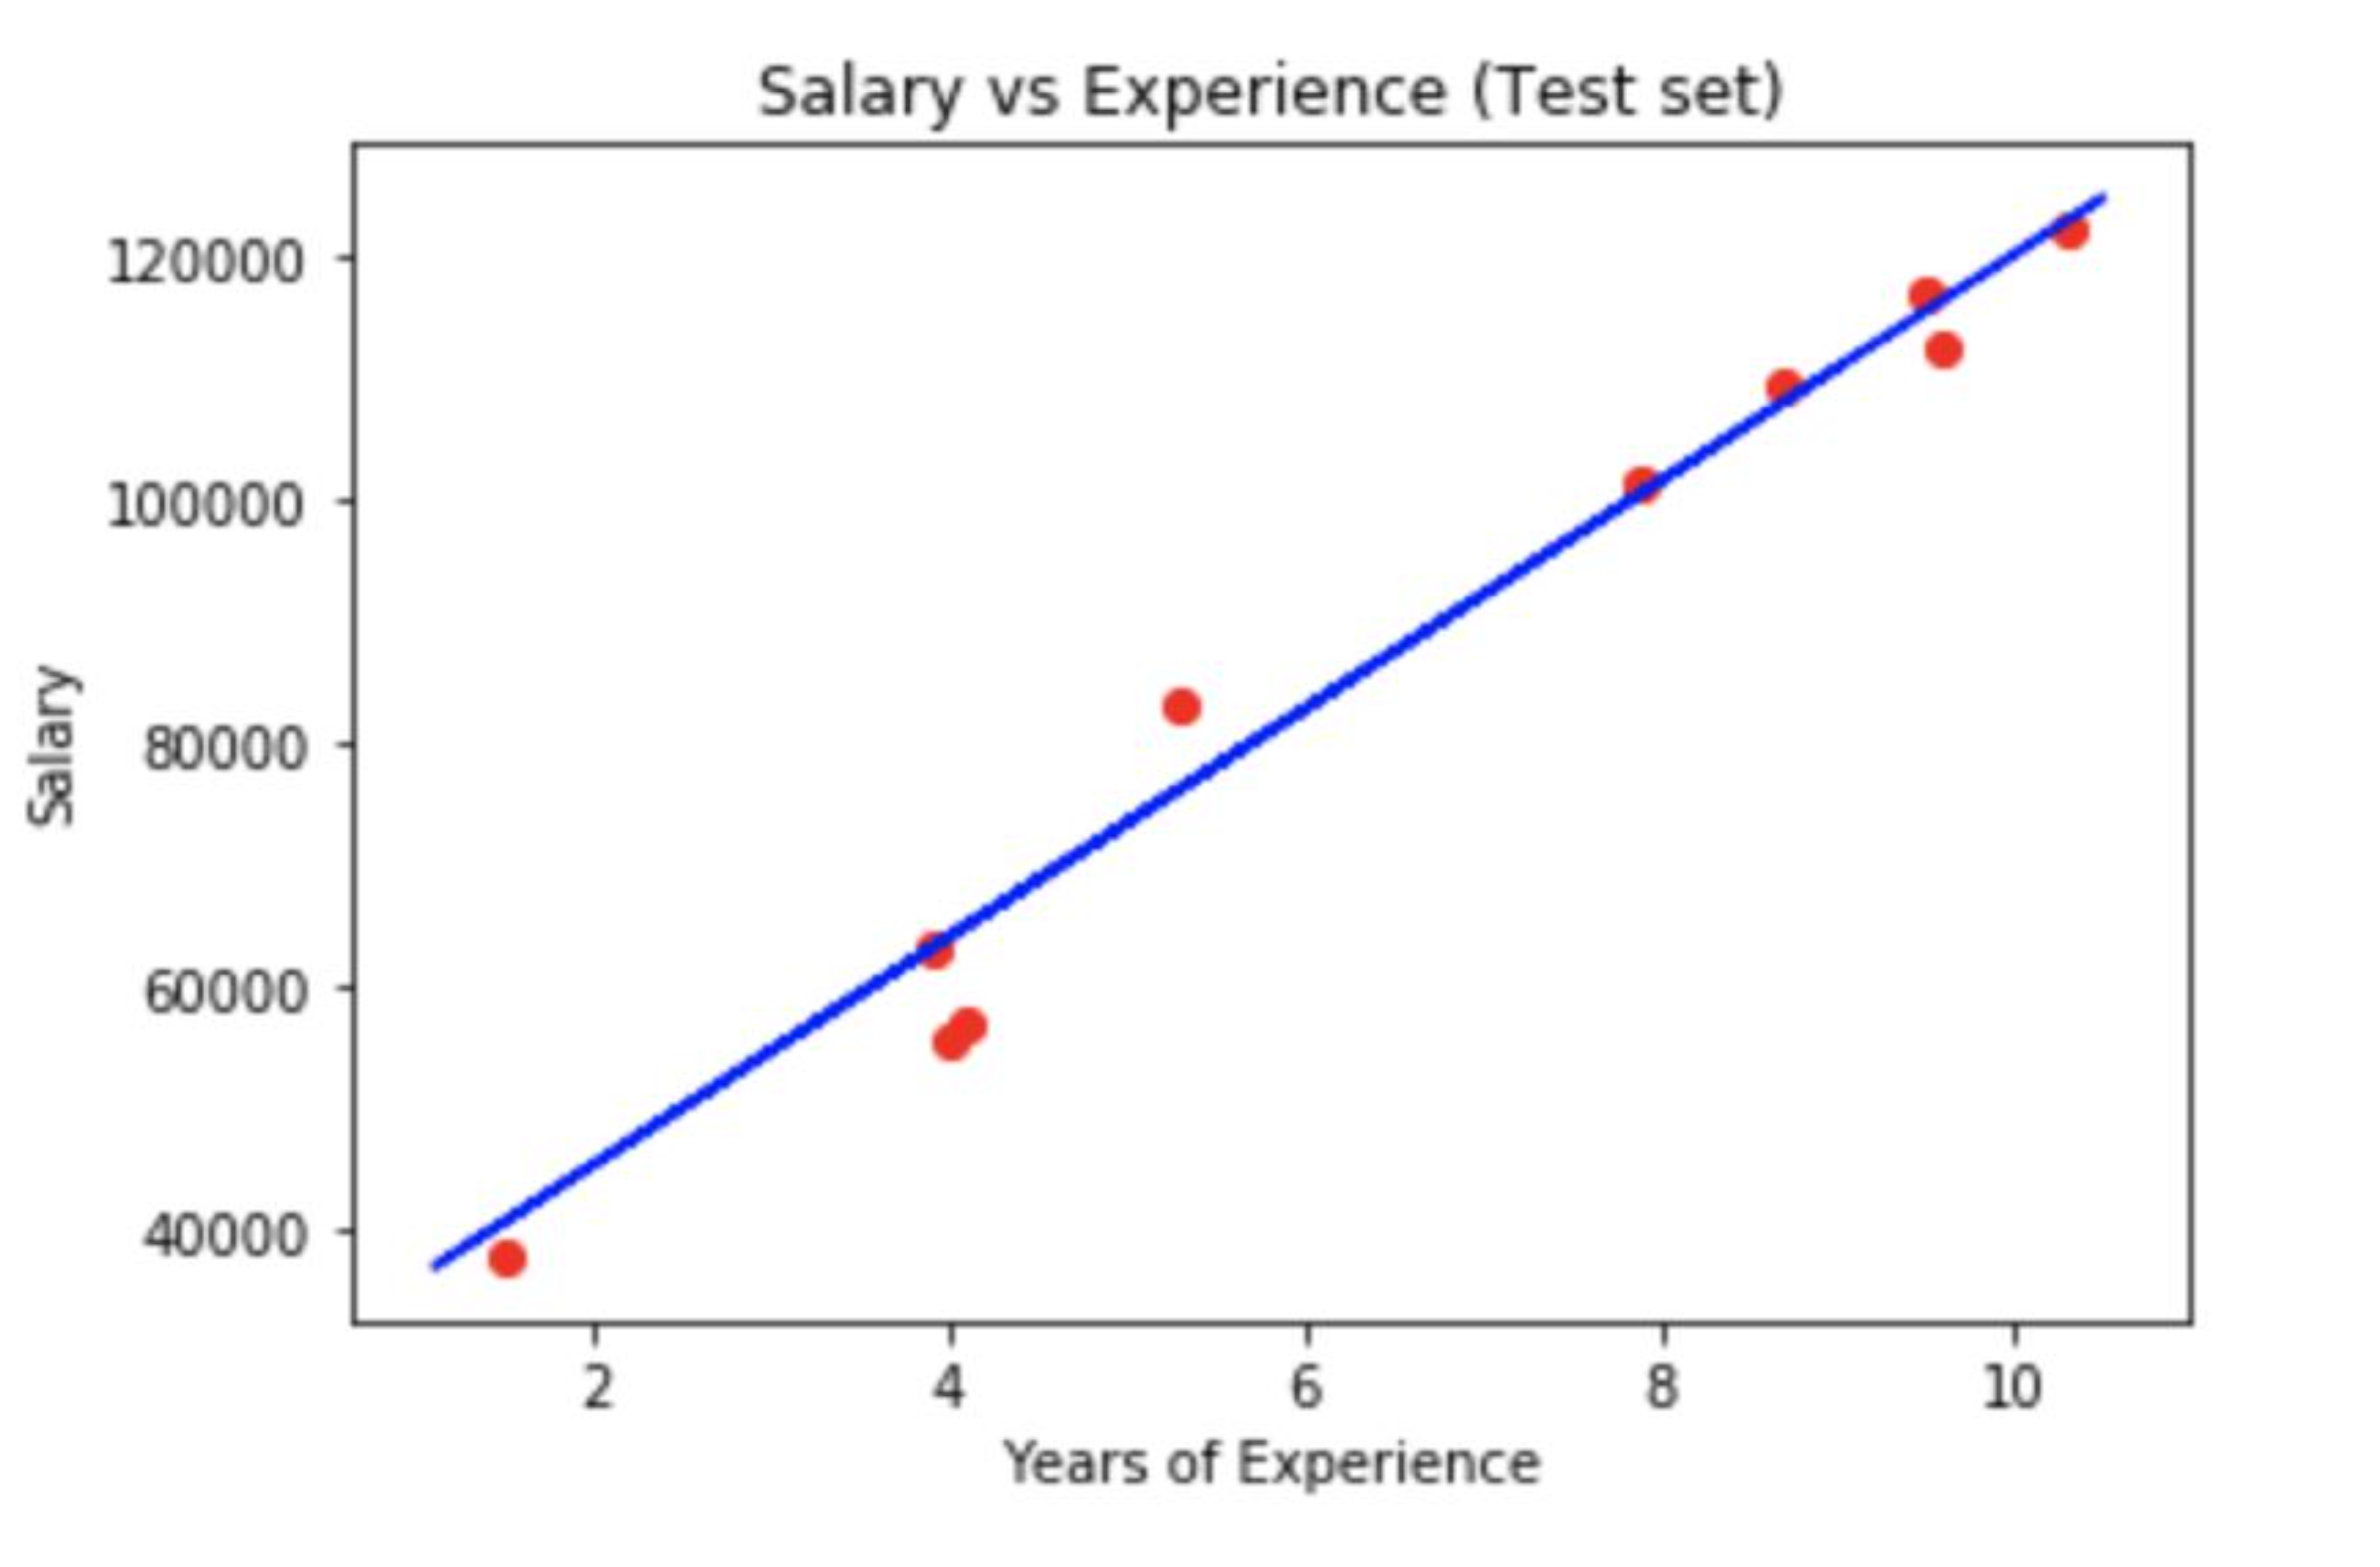
\includegraphics[width=100mm]{images/final.png}}

\nextexercice
\newpage

\end{document}